% Preamble
\documentclass[11pt]{report}

% Packages
\usepackage[a4paper]{geometry}
\usepackage[english]{babel}
\usepackage[indent=20pt]{parskip}
\usepackage{graphicx}
\usepackage{hyperref}
\usepackage{tabularx}
\usepackage{siunitx}
\usepackage{wrapfig}
\usepackage{tikz}
\usepackage{listings}

% textidote: ignore begin
\graphicspath{ {./images/} }

\hypersetup{pdfborder=0 0 0}

\usetikzlibrary{shapes.geometric, arrows}

\tikzstyle{startstop} = [
rectangle,
rounded corners,
minimum width=3cm,
minimum height=1cm,
text centered,
draw=black,
fill=red!30
]

\tikzstyle{io} = [
trapezium,
trapezium left angle=80,
trapezium right angle=100,
minimum width=3cm,
minimum height=1cm,
text centered,
text width=3cm,
draw=black,
fill=blue!30
]

\tikzstyle{process} = [
rectangle,
minimum width=3cm,
minimum height=1cm,
text centered,
text width=3cm,
draw=black,
fill=orange!30
]

\tikzstyle{decision} = [
diamond,
minimum width=3cm,
minimum height=3cm,
text centered,
draw=black,
fill=green!30
]

\tikzstyle{function} = [
circle,
minimum width=2cm,
minimum height=2cm,
text centered,
draw=black,
fill=yellow!30
]

\tikzstyle{arrow} = [thick,->,>=stealth]

\tikzstyle{line} = [thick]
% textidote: ignore end

% Document
\title{P1}
\author{Group 4}

\begin{document}
    \maketitle

    % textidote: ignore begin
    \tableofcontents
    % textidote: ignore end

    \chapter{Problem analysis}\label{ch:problem-analysis}

\section{Shortcomings of commuting}\label{sec:shortcomings-of-commuting}

This Section will dive into the issue of commuting, encompassing the issue's existence, its potential consequences,
the current perceptions of commuting, and the necessity to define the subject and purpose of addressing this issue.
A crucial facet of this analysis is to shed a light on the concealed costs associated with commuting, which is time,
money, climate and health impact, empowering individuals to make informed travel decisions~\cite{alma9921355859805762}.
% TODO Find `Enda, 2011` source and append it to \cite after `alma9921355859805762` (?)

Commuting is a universal challenge that individuals across the globe face daily.
The existence of this problem is deeply rooted in the challenges faced by commuters as they navigate various modes of
transportation, from personal vehicles to public transit.
This existence is compounded by the prevalent issues of traffic congestion, stress, time inefficiency, heightened
greenhouse gas emissions, and financial strain.
These problems are accentuated by the continued urbanization and centralization of job opportunities.
As our cities expand, more individuals are drawn to urban cities in search of employment opportunities, resulting in a
growing commuting dilemma.
% TODO Find `Enda, 2011` source and insert it after `dilemma` and before `.` (?)

The consequences of the problem remaining unaddressed will have a profound impactful, affecting individuals, society,
and the environment.
Traffic congestion, particularly in urban areas during peak hours, results in reduced productivity, increased fuel
consumption, and growing frustration among commuters.
Extended commutes also lead to stress, anxiety, and various health-related issues.
The time spent in daily commutes consumes significant portions of daily life, diverting valuable time from work,
rest, and personal life.
Moreover, the reliance on diesel cars intensifies air pollution and contributes to the pressing challenge of
climate change, raising ecological concerns.
The financial burden of commuting, encompassing expenses such as fuel, vehicle maintenance, public transportation fares,
and parking fees, places individuals and families under considerable financial strain~\cite{alma9921355859805762}.
A wide range of individuals, such as kids, teen, adults and elders, often navigate their daily commutes through a
combination of personal cars, public transportation, cycling, and walking.
This experience is characterized by crowded public transit, traffic congestion, and a perpetual struggle to manage time
effectively.
The daily challenges of commuting frequently lead to physical and mental exhaustion, even in the face of urban growth.
% TODO Find `Enda, 2011` source and insert it after `planning` and before `.` (?)
It encompasses various transportation modes, including personal vehicles, public transit, cycling, and walking.
Additionally, it scrutinizes the societal and individual impacts of commuting, encompassing both positive and negative
aspects.
This subject holds relevance for people who must manage their work or academic pursuits alongside their daily
commutes~\cite{alma9921355859805762}.

The purpose of this analysis is to raise awareness about the profound impact of commuting on individuals, society, and
the environment.
By shedding light on the concealed costs of commuting, which include time, money, and climate and health effects, the
analysis aims to empower individuals to make well-informed decisions regarding their daily travel routines.
Furthermore, it underscores the necessity for innovative solutions and policy changes to mitigate negative consequences
and promote sustainable and efficient transportation options that can make the lives of students and working
professionals more manageable.
% TODO Find `Enda, 2011` source and insert it after `manageable` and before `.` (?)

Often the average individual, frequently underestimate the concealed costs associated with their daily journeys:

\begin{itemize}
    \item \textbf{Time}: Commuting consumes a substantial portion of daily life that could be more productively
    allocated to work, leisure, or personal activities, thus influencing people's work and personal lives.
    \item \textbf{Money}: The expenses associated with commuting, including fuel, maintenance, parking fees, and public
    transportation fares, accumulate over time and impact individuals' financial stability, an issue that particularly
    affects the lower working class.
    \item \textbf{Climate Impact}: Commuting contributes to carbon emissions and air pollution, exacerbating
    environmental challenges, and underscores the significance of environmentally conscious transportation
    choices~\cite{alma9921355859805762}.
    \item \textbf{Health Impact}: The stress and anxiety associated with commuting, particularly in urban areas, can
    lead to various health issues, including high blood pressure, heart disease, and
    depression~\cite{commuting-and-your-health}.
\end{itemize}

\section{Make people aware of how much money, time, climate they are using on commuting}
\label{sec:make-people-aware-of-how-much-money-time-climate-they-are-using-on-commuting}

A study from Denmark’s statistic clearly shows that out of the around three million people in the workfoce only
185 thousand people doesn't commute to work.
This means that \(93.88\,\%\) of the working population commute to work in Denmark~\cite{erhvervspendling2021}.

People are generally uninformed about how much emissions they are helping to produce while travelling in their
desired commuting option.
The desired preference of the commuting can change the way people commutes.
A study made in 2021 on commuting showed which transport option users would pick depending on what their preferences
were.
In this study, we can clearly see that public transport is preferred when the priority is saving time, cost or being
environmentally friendly while walking or cycling were more preferred when health was the priority~\cite{spark2023}.

This is interesting because if people had the opportunity to select either economy, time or sustainability as a
preference when commuting they could use alternative transport options.
Furthermore, this could possibly promote sustainable commuting.
This may be important as sustainable living is becoming more trending than ever.
This may be a direct result of people becoming more aware of how their choices can have an effect on the environment they
live in.

Research done by Capgemini research shows a correlation between sustainability and significant business benefits.
This means that customer loyalty and revenue increases by having a focus on being sustainable~\cite{capgemini2020}.
The enlarged focus on sustainability stems from the new youth, as they prioritize sustainability more than millennials.
% Ovenstående sætning mangler reference.

Commuting can also influence mental health and well-being as it can cause an increase in stress level.
One study suggests that one of the factors increasing stress levels is that the commuters have a difficulty in
appreciating their way of commuting.
% Hvad betyder ovenstående sætning??

The author furthermore explains that the governments must prioritize what the commuters prefer.
These workers can have an incline in stress levels as they have deadlines and specific meeting times that need to be
reached in time~\cite{koslowsky2013}.
By this we can derive that having the opportunity to travel to your destination as fast as possible can be beneficial
for the health.

Another study on 208 people who were rail commuters in New York showed that the longer time that they commuted the more
their cortisol level increased.
This means that time duration of commuting is an important factor for some users.
Therefore, it is essential that people commuting can have an influence on time spent commuting.

Another critical aspect is how commuting effect the economy of people.
A study shows that the average American citizen spends \SI{8466}[\$]{} on co commute expenses.
% Hvad er co commute?
There is a different cost involved in the commute depending on which transport options are used.
For example, \(76\,\%\) of commuters use their personal vehicle~\cite{bankrate2023}.
% Mangler reference på ovenstående tal.
They may also have some extra expenses besides just the buying price of the car.
The average driver spends \SI{1771}[\$]{} on full car insurance and furthermore they spend money on car maintenance
and occasionally after 5000 miles they need to get their vehicles' oil changed.
This could be a challenge as research shows that 1 out of 3 drivers can't afford sudden unexpected car repairs.
The study also suggests that using public transport, bike or scooter to work will cost less~\cite{bankrate2023}.
This change could be difficult as commuting in a personal vehicle could be much more time efficient.

The same study showed that the working poor who commuted by public transport spend \(10\,\%\) of their income on
commuting compared to \(21\,\%\) when commuting in their car.
The working poor prefer saving money because this means they can spend a larger portion of their income on other
relevant expenses like food, healthcare, household supplies and saving for the future.
From this, it is apparent that especially the poorer people would prefer having the opportunity to
commute by cost preferences.
This could improve their economy as the working poor tend to use the least expensive options of commuting, like
carpooling, van pooling, biking, walking and public transport.
Comparing this to people with higher income they are more inclined to spend more on commuting~\cite{bankrate2023}.

% TODO Reference figure in a more meaningful way, as it is not neccesary to include in the current state of the analysis
\begin{figure}
    \centering
    \includegraphics[width=\textwidth]{stats}
    \caption{A picture of a gull.}
    \label{fig:figure}
\end{figure}

% TODO Reference figure in a more meaningful way, as it is not neccesary to include in the current state of the analysis
\begin{figure}
    \includegraphics[width=\textwidth]{stats-2}
    \caption{A picture of a gull.}
    \label{fig:figure2}
\end{figure}

People have been commuting since the beginning of humanity.
From fetching berries in the forest to fighting in wars.
In more recent human history commuting encapsulates something more complex.
Before the information age in the 20\textsuperscript{th} century and before cars and busses were mainstream transport vehicles, most people traveled on foot or on animal to and from work.

\section{Target audience analysis}\label{sec:target-audience-analysis}

When working on a large scale project, it is important analyze who the target user-base is.
The problem has to be big enough to affect a large number of users and the solution has to be viable to be used by said
users.

\subsection{Users}\label{subsec:users}

The main concern is about travelling, which covers a wide range of people, as almost everyone travels one way or another
.
Some examples include travelling to work, travelling to school, family visits, or outings with friends.
As this range is too broad we will in the following section narrow the target user-base down.
There are already some solution to this issue, but in the `Extant solutions and their operational mechanisms' section
below, we figured that these already existing solutions are more fit for single trips, rather than every day travelling.
This gap in use case is mainly what we want to focus on, which is why our target audience is \underline{commuters}.

\subsection{Age range}\label{subsec:age-range}

With our user group in mind, we can estimate an age range for commuters.
Commuting means to travel to the same destination and back on a regular basis.
Therefore, our focus on destinations for commuting are either education or work.

In Denmark, primary schools are chosen for students based on the district where the student lives~\cite{primary_school}.
This would exclude them from our target user-base, as we want to focus mostly on long distance commuters.
At shorter distances, we would need to exclude planes, trains, and for people younger than 18, cars, making it a matter
of whether the student should commute by walking or by bike, which are both \unit{CO_{2}} friendly options and trivial
to choose between, making our solution somewhat irrelevant for this age group.

From secondary education however, students can freely pick which high school they want to go to and the closest school
will be chosen for them.
This, however, makes them a candidate for our user-base, as there are not as many high schools as there are primary.
Many students therefore have a longer commute to school.
Secondary education starts when the student is 16 years old~\cite{secondary_school}.
Our cutoff in the age range would be retirement, as we assume that retired individuals will no longer be commuting in
retirement.
The retirement age in Denmark is 66-68 years of age~\cite{retirement}, making our age range
\underline{between 16 and 68 years}.

The age range is rather large as the user-base includes a large part of the population, which makes our solution rather
difficult, as we have to accommodate it for teenagers as well as adults and the elderly.
The program will therefore have to tailored to all these age groups.

\subsection{Persona}\label{subsec:persona}

To further analyze our user-base, we decided to use the \textit{persona} method.
It works by creating fictional people with different fictional issues and look into how our solution could help them
with their issue.
Below are three personas, with their images generated by GAN AI~\cite{thispersondoesnotexist}, where each of them
cover different age groups and have distinct characteristics related to the main problem.

% Persona skal vaere i bilag

\renewcommand{\arraystretch}{1.5}

\noindent
\begin{tabularx}{\textwidth}{ | l X | }
    \hline
    &                                               \\
    & \includegraphics[width=0.25\textwidth]{asger} \\
    Name       & Asger Johansen                                \\
    Age        & 28 years old                                  \\
    Occupation & Designer                                      \\
    What's important & For Asger it is important to spend his days to the fullest.
    He is very outgoing, so he goes out with people after work.
    He hates having to stay overtime. \\
    Current problem & Asger just got a new job offer, but it's in another city.
    He isn't sure whether to move out or to commute there.
    He is also afraid of losing his free time if he has to travel. \\
    Potential solution & We would want to make a program, where Asger could calculate how long it'd take to commute from
    where he lives to the new job.
    He could compare different forms of transport and decide whether it's worth it to commute or if he should move out
    instead. \\
    \hline
\end{tabularx}

\noindent
\begin{tabularx}{\textwidth}{ | l X | }
    \hline
    &                                                  \\
    & \includegraphics[width=0.25\textwidth]{josefine} \\
    Name       & Josefine Madsen                                  \\
    Age        & 19 years old                                     \\
    Occupation & Student                                          \\
    What's important & For Josefine it is important to look after the nature.
    She's been taught to think green since she was little, so she doesn't like taking public transport and doesn't want
    to drive a gas car. \\
    Current problem & Josefine is starting university, but she lives outside the city.
    She is considering whether to take the S-train, the train or a bus to university.
    She is also considering buying an electric car. \\
    Potential solution & We would want to make a program, where Josefine could calculate how much the emissions is made
    from different forms of transport.
    She can then compare them and choose what works best for her. \\
    \hline
\end{tabularx}

\noindent
\begin{tabularx}{\textwidth}{ | l X | }
    \hline
    &                                                \\
    & \includegraphics[width=0.25\textwidth]{martin} \\
    Name       & Martin Jensen                                  \\
    Age        & 34 years old                                   \\
    Occupation & Factory worker                                 \\
    What's important & For Martin it is important to live a carefree life.
    He has a family and friends at work, so he's pretty happy with himself. \\
    Current problem & Martin drives a gas car to work, but he wants to change that for the sake of the environment.
    He has gotten used to the comfort of his car, but can't afford an electric car.
    He wonders if public transport could match that. \\
    Potential solution & We would want to make a program, where Martin can figure out what forms of public transport are
    most comfortable and most climate friendly. \\
    \hline
\end{tabularx}

\section{Context}\label{sec:context}

Commuting is one of the staples, so to speak, of modern life, and a central part of the post-modern industrialized
society.
As cities rapidly grew after the industrial revolution and more and more large-scale workplaces became the norm in
cities, people started commuting to work from suburban areas to the city.
In the early stages of this development in the beginning and middle of the 20th century, commuting was a rather simple
task: People just had to get to work in the mornings and back home in the evenings.
Nowadays, the complexity of commuting has increased drastically with many additional factors having to be considered,
e.g., how big of a carbon footprint is acceptable for me?
This question especially became relevant in recent times due to the increasingly noticeable effects of climate change
and the scientific evidence that increased \unit{CO_{2}} emissions greatly contribute to climate change.
Other questions the modern-day commuter might ask themselves are: Do I need/want to commute every day, or is it ok if I
work from home part of the week?
What should be the balance between cost and environmental protection?
Do I live in an area where the availability of public means of transportation is scarce, so I am more inclined to use a
car?
One of the simpler questions someone that considers commuting could ask themselves is merely: What commuting route
should I choose?
With the advent of the digital age and smartphones, the answer to this question have become commuting planner
applications, that have become increasingly popular in recent years, helping individuals plan their daily commutes
efficiently and minimize travel-related stress.
These applications offer various features and functionalities, but they often have shortcomings that prevent the
commuter from more advanced planning strategies, including the lack of easy access to cost and environmental impact
information, e.g., how much \unit{CO_{2}} will be spent on a trip, how much a trip will cost, as well as limited user
control over how these factors are weighed in route calculations.
Existing solutions include the (mostly) worldwide available Google Maps, the popular Danish Rejseplanen service and a
couple of other mobile and web applications that are not location-bound but can be used internationally, like
\url{https://commute.org/}.
We will now look at some existing solutions and discuss their shortcomings to better understand the root of the problem.

\begin{figure}
    \centering
    \includegraphics[width=\textwidth]{images/google-maps}
    \caption{Google Maps web UI.}
    \label{fig:figure6}
\end{figure}

\subsection{Google Maps}\label{subsec:google-maps}

The above-mentioned application is a widely used travel and commuting planner that provides detailed navigation and
route information and can also be seen in Figure~\ref{fig:figure6}.
While it offers estimated travel time and distance, it lacks a direct and user-friendly way to determine the cost of the
trip or the \unit{CO_{2}} footprint.
Users cannot easily access information about how much money the trip will cost, as Google Maps does not integrate with
financial or payment apps to calculate expenses like tolls, fuel, or public transportation fees.
This makes sense since Google tries to target a large international audience with the application, making is difficult
or nearly impossible to cover every localized payment solution or traveling restriction.
Similarly, it does not provide real-time data on the \unit{CO_{2}} emissions associated with the chosen route, making it
challenging for users to make informed decisions about their environmental impact.

\begin{wrapfigure}{l}{0.5\textwidth}
    \begin{center}
        \includegraphics[width=0.4\textwidth]{images/google-maps-options}
    \end{center}
    \caption{Google Maps web UI options.}
    \label{fig:figure7}
\end{wrapfigure}

Users have very limited control over how cost and environmental factors are weighed in route calculations, as Google
Maps primarily focuses on travel time and distance.
The only available selection options, as can be seen in Figure~\ref{fig:figure7}, are preferences for means of
transportation and whether the route should be calculated with ``fewer transfers'', ``less walking'' or ``wheelchair
accessible'', where all three of the options seem to be tailored towards people with restricted mobility.

\subsection{Rejseplanen}\label{subsec:rejseplanen}

In Denmark, the most popular commuting planner application by far is Rejseplanen.
This application, just like Google Maps, is both available as a web and mobile application.
The app lets the traveler or commuter to enter trip starting and ending locations, which it then uses to calculate a
route using public means of transportation or as secondary options as walking routes.
When a route is calculated, the user is presented with a list-like interface from which the details of the trip can be
read; what means of transportation will be used, which lines, what the departure and arrival times are, and if there are
any special restrictions on the trip.
See Figure~\ref{fig:figure8}.

\begin{wrapfigure}{r}{0.4\textwidth}
    \begin{center}
        \includegraphics[width=0.3\textwidth]{images/rejseplanen-trip}
    \end{center}
    \caption{Rejseplanen mobile UI trip planner.}
    \label{fig:figure8}
\end{wrapfigure}

Getting the price of the trip is possible too, but in a primitive manner that doesn't consider factors such as if the
user is a tourist or a regular resident, which is an important feature since tourists might have different traveling
strategies than regular residents, and additionally tourists might not use the prepaid Rejsekort card, etc.
There is an additional option of adding your Rejsekort ID to the app, so it can calculate the trip price based on your
card plan, but even that feature is kept rather simple, possibly because the Danish transportation authorities also
released the DOT app, whose primary responsibility is exactly that: calculating trip prices and buying tickets.
See Figure~\ref{fig:figure9}.

\begin{figure}
    \centering
    \includegraphics[width=0.5\textwidth]{images/rejseplanen-options}
    \caption{Rejseplanen mobile UI trip planner options.}
    \label{fig:figure9}
\end{figure}

The user can also customize the trip's parameters slightly, e.g., if it's a biking or a walking trip, what the maximum
allowed biking or walking distance should be, whether the user is a ``slow'', ``medium'' or ``fast'' walker (even though
there is no guideline for how fast exactly each of these options is), and a few additional details, but a feature that
definitely lacks is the calculation of the trip’s total \unit{CO_{2}} emissions, which is an important factor in the
modern-day world.

% TODO Make sections, subsections and subsubsections much longer and remove TeXtidote ignore annotation
% textidote: ignore begin
\section{Extant solutions and their operational mechanisms}\label{sec:extant-solutions-and-their-operational-mechanisms}

In this section, we will discuss extant solutions and their operational mechanisms pertaining to the provided problem
statement.
We will analyze prominent software applications in the market, including Rejseplanen, Google Maps, and Apple Maps.

\subsection{Rejseplanen}\label{subsec:rejseplanen2}

We will first take a look at the Danish ``Rejsekort'' application.

\subsubsection{What is Rejseplanen?}

The ``Rejseplanen'' is an online service used in Denmark to plan journeys using public transport.
It is used to find information about routes, timings, prices and ticket purchases for trains, buses, metro, trams and
ferries throughout the country~\cite{rejseplanen2023}.

With ``Rejseplanen'', you can input your departure point and destination point to get information about the fastest,
cheapest or most convenient way to travel from point A to B using public transport.
The service provides detailed information about the departure times, transfers, expected arrival times and prices.
It also provides any additional information about the delays or canceled departures in the operation of public
transport~\cite{rejseplanen2023}.

\subsubsection{Data sources for Rejseplanen}\label{subsubsec:where-does-rejseplanen-get-their-data-from?}

Rejseplanen is jointly owned by DSB, Movia, Metroselskabet, NT, Midttrafik, Sydtrafik, Fynbus, and BAT\@.
As a result of its ownership by these various transportation service providers, Rejseplanen has access to the data
necessary to determine the most efficient public transport routes.

\subsubsection{What makes Rejseplanen great?}\label{subsubsec:what-makes-rejseplanen-great?}

\begin{itemize}
    \item \textbf{Comprehensive data integration}: Rejseplanen integrates data from various transportation providers,
    thus ensuring up-to-date and accurate information.
    \item \textbf{Very efficient}: Rejseplanen provides a quick and convenient travel plan, saving time for daily
    commuters.
    \item \textbf{User-friendly}: Rejseplanen provides additional features such as filtering out specific trains or
    buses, so your route matches your personal preferences and enhancing the user experience.
\end{itemize}

\subsection{Google Maps/Apple Maps}\label{subsec:google-maps-/-apple-maps}

We will now take a look at the two internationally popular ``Google Maps'' and ``Apple Maps'' services.

\subsubsection{What is Google Maps}

Google Maps is another online service used for travelling.
It is one of the most extensive and detailed mapping databases globally.
Its comprehensive coverage includes even remote areas, making it a go to for travelers and commuters.
Whether you're navigating in unknown areas or exploring remote landmarks, Google Maps is sure to provide accurate
mapping data~\cite{googlemaps2023}.

Google Maps began as a C++ desktop program developed by two Danish software engineers who so happens to be brothers,
Lars Eilstrup Rasmussen and Jens Eilstrup Rasmussen~\cite{googlemaps2023}.

\subsubsection{What is Apple Maps}

Apple Maps is mostly the same as Google Maps, it also has very detailed mapping data.
Apple Maps also provide a navigation function like Google Maps that is with turn-by-turn directions for driving, walking
and public transportation.
It also supports real-time traffic information and alternative routes to help users reach their destination more
efficiently.
Apple Maps can provide various information about shopping centers, restaurants, hotels and gas stations.
Some of that information includes user reviews, photos, contact details and hours of operation.
Google Maps does also provide this kind of information.

Google Maps used to be the default web mapping service for iOS, but they replaced Google Maps with their own version
which is of course Apple Maps now~\cite{applemaps2023}.
% textidote: ignore end

\section{Recommendation systems}\label{sec:recommendation-systems}

In Denmark when using apps to guide your travels, you will have to choose between the different means of transport such
as: by car, train, bus, cycling or walking.
If you wanted to prioritize your climate footprint with these already existing apps you would have to research how much
a specific means of transportation pollutes.
Another situation is the economics of one's travel.
Instead of individuals having to calculate for themselves how much money they would spend on a specific travel type,
it could be done automatically.
To make it as easy as possible to make an informed decision for the users of our program, we want to automate many of
these calculations, such that the users can get an overview of their situation in a fast and easy way.

To accompany this, the authors will build a system that shows the routes that the user would want to travel by based on
their personal preferences.
This can also be called a recommendation system (RS).
RS is something we all use every day, when browsing a web shop, YouTube or other streaming services.
The goal of an RS is to sort through all available data and assume and present the most useful data to the user.
The close parallel there is between these RS and our problem solution gives rise to a segment explaining RS in more
detail.

A real world example of where this is used is in a movie recommender.
Movies are somewhat easy to classify, as one can look at the genres of different movies for example.
This type of RS works by filtering the movies through genres and is called ''content based filtering'' as seen in.

\begin{figure}
    \centering
    \includegraphics[width=\textwidth]{content-filtering}
    \caption{Content filtering. \cite{content_based_filtering}}
    \label{fig:figure3}
\end{figure}

An example would be user a watching an action movie, movie A, and the system would then remember user a's preferences
and recommend another action movie, movie B, to the user as seen in ~\ref{fig:figure3}.
This is a very simplified version of content filtering as they usually utilize multiple attributes from both the content
and the user.
In the context of a movie recommender this could be both the themes, the producer, the actors etc.
In content filtering, a user's history and interactions is used to create the profile for the RS to give suggestions.
Although content filtering is better than recommending random movies, it does not take human tendency to have changing
opinions and tastes into consideration.

Another type of filtering is Collaborative filtering (CF).
CF works by comparing users with each other.
This means that CF groups users by similarities in their watched movies, and then suggests movies from the users group,
as seen in~\ref{fig:figure4}.

\begin{figure}
    \centering
    \includegraphics[width=\textwidth]{collaborative-filtering}
    \caption{Collaborative filtering. \cite{collaborative_filtering}}
    \label{fig:figure4}
\end{figure}

Using CF does not limit the recommendations to genres or other attributes that the program already know the user
watches.
It can also recommend things from other genres, which would not have been recommended by the content filter.
Generally for both these types of filters, they need a lot of information about both the user and the content.
This is however out of the scope of this project.
While content filters and collaborative filters are versatile in their use, the goal for this project is to use them to
recommend routes and make the user aware of both the monetary impact and the impact on our climate as well as
recommending the best routes.
In this context, it would be more logical and simpler to get the users preferences directly through what could be a
questionnaire, rather than relying on behavior analysis.
The attributes one could use for the filters are straight forward, as they could be climate impact, cost, time and
others.
This would however require some analysis to get more useful data out of the routes we generate.
Using a weighted system to measure the results of our program would allow us to choose a specified amount from the top,
and by doing this we will have chosen the most relevant for the users.


    % TODO Make chapter much longer and remove TeXtidote ignore annotation
% textidote: ignore begin
\chapter{Problem statement}\label{ch:problem-statement}
% textidote: ignore end

Now we want to define the problem statement.


\section{Deviation}\label{sec:deviation}

In a modern world interconnected through both highways, rails, airports or roads, where people have the means to take
the climate and other things into account, when planning their routes to work or education.
The issue is that not enough people actually do this.
We believe the reason for this is that there is no easy way to get this information, and by giving them a way through
our app to plan their route for their preferences many more would try it.

% TODO Make section much longer and remove TeXtidote ignore annotation
% textidote: ignore begin


\section{Statement}\label{sec:statement}
% textidote: ignore end

How can we help individuals choose a commuting route that best suits their preferences?

% TODO Make section much longer and remove TeXtidote ignore annotation
% textidote: ignore begin


\section{Under questions}\label{sec:under-questions}
% textidote: ignore end

What can we do to inform commuters about the financial cost, time, comfort or environmental impact that different forms
of transportation can cause.
What are the parameters that affect the choices.
How can we help individuals make a choice on whether to move closer to their place of occupation or to commute from
their current place of living?

    % textidote: ignore begin
\chapter{Method}\label{ch:method}
% textidote: ignore end

\section{How can we help solve this problem?}\label{sec:how-can-we-help-solve-this-problem?}

The goal of this project is to help people understand their travel options, and also help them choose the one most
inline with their preferences.
Making this program would also allow users to plan their journey days before, which would improve traffic flow
overall and quality of life for the consumers.

We gather data from ``rejseplanens'' API such that we can request data about the public transport in Denmark.
We further investigate the environmental factors where we investigate how much \unit{CO_{2}} emission
different car types and public transport types causes per kilometer.

We research how much \unit{CO_{2}} emission different types of cars cause and set them to an average for
the program parameters to make it simpler to calculate routes with less \unit{CO_{2}} emission.
The same goes for public transport.
We research how much \unit{CO_{2}} emission trains, buses and metros emit.

We allow users to make different priorities such as the time of arrival, cost, environmental impact and comfort.
Furthermore, a filter is added where the user is able to set their own priorities.

The user interface (UI) is supposed to be user-friendly, such that it can be used effectively by all
consumers.
The UI we are using for this project is the terminal, which is text-based.
The reason for the choice of our UI is limited by the projects restrictions in which we were recommended to make a
terminal UI instead of another more user-friendly graphical UI\@.

\section{Solution stack}\label{sec:solution-stack}

In the following section, we will take a closer look at the solution stack that the development team has chosen to use
to create the software that will constitute the problem solution.

\subsection{Development team}\label{subsec:development-team}

The development team consisted of seven young computer science students with different levels of previous development
experience.

\subsection{Basic requirements}\label{subsec:basic-requirements}

Before the development team began the development process, a wide variety of basic technological and workflow-related
requirements and constraints were discussed.

The team understood very quickly that high productivity and development efficiency were one of the top priorities for
the task at hand, due to the relatively short deadline, development team size and the complexity of the software's
logic.

Other constraints were identified as well, such as the fact that while every member of the development team had
different levels of experience with different programming languages and technologies, everyone was familiar with the
C programming language.

Finally, coming from a wide range of backgrounds and having different preferences, the individual members of the team
wanted to be able to make individual choices regarding their development setups, while still maintaining project-level
coherency.
Examples of such individual preferences included which development operating system each member would work on (such as
Windows 11, macOS, various Linux distributions, and also Windows Subsystem for Linux (WSL)).
Additionally, individual preferences extended to choices regarding what code editor or intelligent development
environment (IDE) the member would use.
And finally, another constraint dictated by personal preferences was what tools were available for the chosen
development platform, such as compilers, linters, etc.

Those three basic realizations largely dictated all the other choices of technologies, workflows and other development
tools.

\subsection{Version control}\label{subsec:version-control}

When dealing with a software project of this size and complexity, combined with a development team of this size, it is
crucial to be able to collaborate remotely over the internet.
Also, it is paramount that the team is able to trace incremental changes in the software source code.
This is where version control and version control systems come into play.

\subsubsection{Version control system}

For this project, the team selected the \lstinline{git} version control system, which is modern, efficient and
relatively easy to use.
The usage of \lstinline{git} allowed each team member to develop incremental features and changes on their own
development machine and then combine the changes on the \lstinline{main} version control branch.
To further ease the process and make individual development fully independent, a server was needed to which the
individual members' contributions could be uploaded.
For this task, \href{https://github.com/}{GitHub} was chosen, and a public code repository was created using the private
GitHub account of one of the team members.
The repository can be found here: \href{https://github.com/audio-engineer/aau-p1-software}{aau-p1-software}.

\subsubsection{Branching model}

Modern version control using \lstinline{git} relies on the idea of \textit{branching}.
\textit{Branches} consist of a series of \textit{commits}, which are snapshots of the source code taken at arbitrary
times by the developers while working on their development machines.
The team decided that the easiest approach to branching would be a model based heavily on \textit{trunk-based
development}~\cite{trunk-based}, which is a simple model where all changes from individual branches are merged directly
into the project's \lstinline{main} branch without additional branching complexity.
Additionally, to keep the development routines as simple and efficient as possible, it was decided that each developer
would have their own branch on which they would continuously commit their individual contributions.
Those branches were then continuously uploaded (\textit{pushed} in \lstinline{git} terminology) to GitHub, where they
were merged into the \lstinline{main} branch.
Each time after a merge was completed, the contributor in question's branch was reset to match the \lstinline{main}
branch, upon which the development cycle was resumed.

We will take a closer look at how it was implemented practically in the Section~\ref{sec:workflows-and-routines}.

\subsection{Development systems and tools}\label{subsec:development-systems-and-tools}

As previously mentioned, the team's personal development setup preferences varied, not least in the choice of code
editor or IDE, and development machine operating system.
Simultaneously, it was determined that to maximize efficiency, some project configurations and other related settings
would have to be shared across development machines and operating systems.
This was deemed necessary to prevent that each developer would have to set up their local development environment
from scratch.
To mitigate this issue, some sort of configuration sharing was necessary to be introduced into the development flow.
Luckily, a majority of the developers were already familiar with the IDE vendor JetBrains' products, which offer great
support for shared configurations~\cite{shared-config}.
Therefore, a shared configuration was added to the source code repository, which was then read by each developer's
IDE upon opening the project.
Examples of configurations that were shared include code indentation and bracket placement style, unit test runner
configuration, text encoding, required IDE plugins and code linting settings.

\subsection{Programming languages}\label{subsec:programming-languages}

As was mentioned in the Section~\ref{subsec:basic-requirements}, the C programming language was the single
programming language that all developers in the team were familiar with, which is one of the primary reasons why it was
chosen as the development language.

Another reason was the flexibility that C offers: It can be developed and compiled for a wide range of target systems.
In other words, C offers cross-platform compatibility both from development and distribution perspectives.

It was also decided early on that the solution application would be a console application, and C also has the advantage
that it is an excellent language for console application development.

Finally, C has been on the market for many decades and is a very well-established language with exceptional tooling and
availability of libraries, compilers, IDEs, and frameworks that support it, making it a good choice for many tasks.

But while C made up the majority of the source code, it also turned out to be necessary to introduce C++ into the
project, due to the usage of the \textit{GoogleTest} unit testing library.
GoogleTest is originally built for usage with C++, but can easily be adopted to be used with purely C-based projects,
only requiring slight modifications to how the project is built and how the tests are written.
Also, luckily GoogleTest is almost exclusively built on macros, which made writing tests a lot easier for the team,
since only very little or almost no C++ syntax had to be learned.
This will be further discussed in the Section~\ref{subsec:testing}.

\subsection{Integrations}\label{subsec:integrations}

// REST service, Rejseplanen API

\subsection{Build system}\label{subsec:build-system}

One of the disadvantages of C, though, is that it requires a solid and substantial ecosystem of build tools and
compilers around the C source code to be able to build the distribution-ready application.
One approach would be to let each developer set up their own build system to be able to compile the source code on their
local development environment, and then later decide on a \textit{master} compilation machine where the distribution
version would be compiled.
But the development team chose an approach where the build configuration was built into the source code itself, making
it easy to share it across local development environments.
This also allowed each developer to build the software using the same build parameters.

The primary tool picked to solve this task was CMake, which is a build automation tool that generates build
configuration files based on a common project configuration.

CMake also has the advantage that it can prepare the compilation machine for compilation by searching for compilation
dependencies aka ``dependencies of dependencies'' without which the compilation would fail.
For this purpose, the team made use of the \lstinline{pkg-config} CMake integration. \lstinline{Pkg-config} is a tool
that searches the compilation machine exactly for those prerequisite dependencies to make sure that all direct
dependencies and if they are not found, the compilation is aborted.
If they are, on the other hand, found, the application compilation is resumed and completed.

% TODO Insert CMake dependency, compilation and linkage flowchart

Furthermore, CMake also allows for the addition and management of external software dependencies such as libraries
and frameworks, which will be discussed in the Section~\ref{subsec:libraries-and-frameworks}.

\subsection{Libraries and frameworks}\label{subsec:libraries-and-frameworks}

% TODO Add more content to this subsection
// cURL, cJSON, OpenSSL

\subsection{Code style and quality}\label{subsec:code-style-and-quality}

When working on larger scale software projects where more than one developer is involved, it is also crucial to keep the
source code readable, maintainable and coherent to be able to easily develop and refactor it later.
For this reason, the team decided to use a common code style and use tools to ensure that this style was complied with.
As a baseline, it was decided that the Google C++ Style Guide~\cite{google-style} would be used for basic stylistic
features such as function, data and file naming conventions, an indentation width of two spaces, bracket placement, etc.
While the Google C++ Style Guide is, as the name suggests, made for C++ projects, it can easily be adopted for usage
with C projects by simply adhering only to the style guidelines that regard features that both C++ and C share.

To assist the developer team with adhering to those guidelines, the \textit{Clang-Format}~\cite{clang-format} and
\textit{Clang-Tidy}~\cite{clang-tidy} tools provided by the \textit{Clang} compiler were used to automatically lint
the code for breaches of style.
This process was made even easier due to the seamless integration of these tools into the JetBrains CLion IDE that was
used by a majority of developers, which made it possible to lint the source code while writing it.

// ClangFormat, ClangTidy, EditorConfig, Google C++ Style Guide, pull requests and code reviews.

We will take a closer look at how it was implemented practically in the next Section~\ref{sec:workflows-and-routines}.

% textidote: ignore begin

\subsection{Testing}\label{subsec:testing}

% TODO Add more content to this subsection
// Unit tests, GoogleTest

\subsection{CI/CD}\label{subsec:ci/cd}

% TODO Add more content to this subsection
// GitHub Workflows/Actions

\subsection{Target systems}\label{subsec:target-systems}
% textidote: ignore end

% TODO Add more content to this subsection
// Cross-platform (Windows, macOS, Linux)

\section{Workflows and routines}\label{sec:workflows-and-routines}

In this section, we will discuss the development team's routines and workflows to gain a better understanding of how
the development process looked like.
The team's workflow for both the program and the report consisted of collaboration, communication, and version control.
Microsoft Teams was used for communication, Trello was used to assign tasks, and GitHub was used for the development of
the project.
Discussions were held in person and Microsoft Teams.
After the discussions, the team would create Trello cards for the task and assign them to individual members.
The GitHub repository has separate branch for each member of the team.
The team would work on their personal branch and then create a Pull Request with the purpose to merge the changes to the
main branch.
The Pull Request would then have to be reviewed by at least 2 other members before it could be merged.
After the merge, the person responsible for the changes will reset their branch and reuse it for the next task.
This workflow was used for both the program and the report.

The team had a weekly meeting with the supervisor, where the team would discuss the progress of the project.
Every meeting would start with a Code Review, where the team would go through the program and discuss the changes made
since the last meeting.
Occasionally, the team would also use the Scrum method to catch up on the progress of the project.
The team would discuss what they had done since the last meeting, what they were currently working on, and what they
would do next.

% TODO Add content to this section and remove `textidote: ignore begin/end`
% textidote: ignore begin
\section{Software project structure}\label{sec:software-project-structure}
% textidote: ignore end

It was decided to make use of an adopted version of the \textit{Pitchfork Layout}~\cite{pitchfork-layout}.


    % TODO Add a lot of text to this chapter and remove TeXtidote ignore annotation around the \chapter command
% textidote: ignore begin
\chapter{Problem solution}\label{ch:problem-solution}
% textidote: ignore end

% textidote: ignore begin
\section{Software Requirements Specification}
% textidote: ignore end

The outline of the requirements of the program is divided into two categories; hard requirements and soft requirements.

\section{Flowchart of the program}

Hello world!

% textidote: ignore begin
%-----------------------------------------------------------------------------------------------------------------------
\subsection{Main}
\noindent
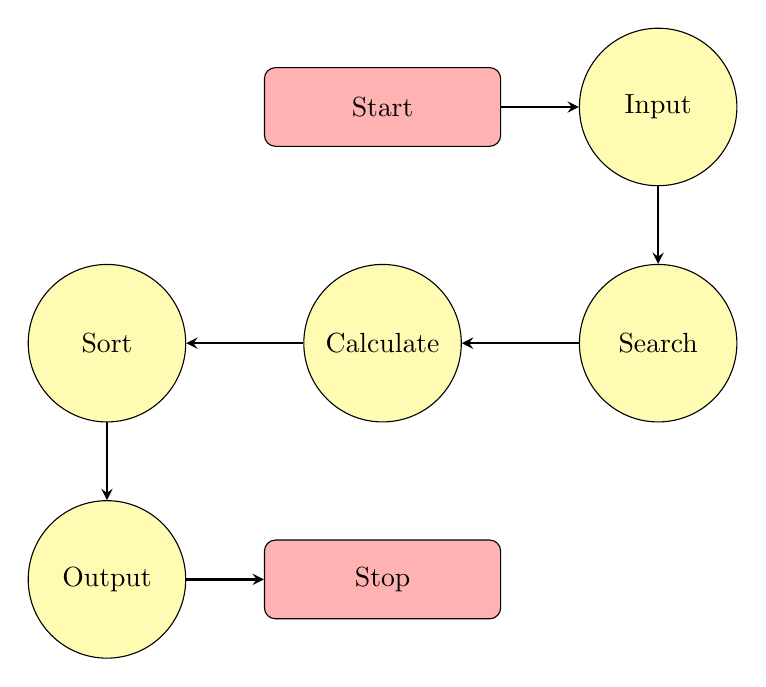
\begin{tikzpicture}[node distance=2cm]

\node (start) [startstop] {Start};
\node (func1) [function, right of=start, xshift=1.5cm] {Input};
\node (func2) [function, below of=func1, yshift=-1cm] {Search};
\node (func3) [function, left of=func2, xshift=-1.5cm] {Calculate};
\node (func4) [function, left of=func3, xshift=-1.5cm] {Sort};
\node (func5) [function, below of=func4, yshift=-1cm] {Output};
\node (stop)  [startstop, right of=func5, xshift=1.5cm] {Stop};

\draw [arrow] (start) -- (func1);
\draw [arrow] (func1) -- (func2);
\draw [arrow] (func2) -- (func3);
\draw [arrow] (func3) -- (func4);
\draw [arrow] (func4) -- (func5);
\draw [arrow] (func5) -- (stop);

\end{tikzpicture}
%-----------------------------------------------------------------------------------------------------------------------
\subsection{Input}
\noindent
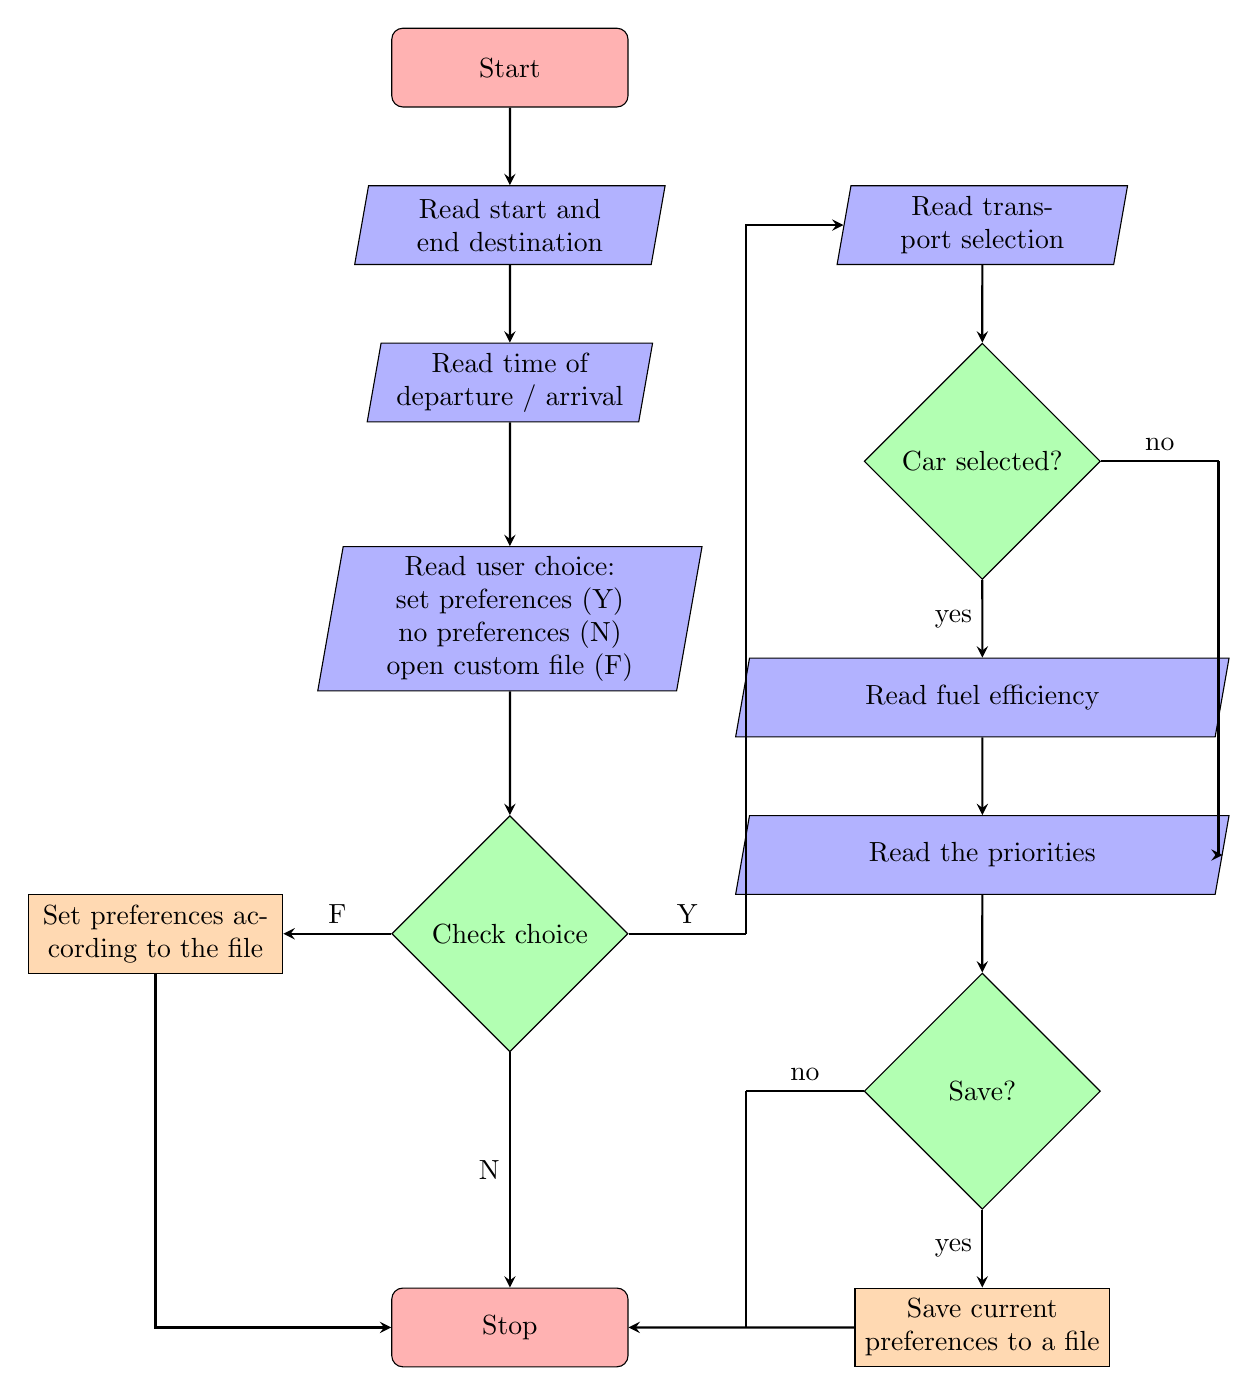
\begin{tikzpicture}[node distance=2cm]

\node (start) [startstop] {Start};
\node (in1)   [io, below of=start] {Read start and end destination};
\node (in2)   [io, below of=in1] {Read time of departure / arrival};
\node (in3)   [io, below of=in2, text width=4cm, yshift=-1cm] {Read user choice:\\ set preferences (Y)\\ no preferences (N)\\ open custom file (F)};
\node (dec1)  [decision, below of=in3, yshift=-2cm] {Check choice};
\node (pro1)  [process, left of=dec1, xshift=-2.5cm] {Set preferences according to the file};
\node (in4)   [io, right of=in1, xshift=4cm] {Read transport selection};
\node (dec2)  [decision, below of=in4, yshift=-1cm] {Car selected?};
\node (in5)   [io, below of=dec2, yshift=-1cm] {Read fuel efficiency};
\node (in6)   [io, below of=in5] {Read the priorities};
\node (dec3)  [decision, below of=in6, yshift=-1cm] {Save?};
\node (pro2)  [process, below of=dec3, yshift=-1cm] {Save current preferences to a file};
\node (stop) [startstop, below of=dec1, yshift=-3cm] {Stop};

\coordinate [right of=dec1, xshift=1cm] (ph1);
\coordinate [left of=dec3, xshift=-1cm] (ph2);
\coordinate [below of=ph2, yshift=-1cm] (ph3);
\coordinate [right of=dec2, xshift=1cm] (ph4);

\draw [arrow] (start) -- (in1);
\draw [arrow] (in1) -- (in2);
\draw [arrow] (in2) -- (in3);
\draw [arrow] (in3) -- (dec1);
\draw [arrow] (dec1) -- node[anchor=south] {F} (pro1);
\draw [arrow] (pro1) |- (stop);
\draw [arrow] (dec1) -- node[anchor=east] {N} (stop);
\draw [line] (dec1) -- node[anchor=south] {Y} (ph1);
\draw [arrow] (ph1) |- (in4);
\draw [arrow] (in4) -- (dec2);
\draw [arrow] (dec2) -- node[anchor=east] {yes} (in5);
\draw [arrow] (in5) -- (in6);
\draw [line] (dec2) -- node[anchor=south] {no} (ph4);
\draw [arrow] (ph4) |- (in6);
\draw [arrow] (in6) -- (dec3);
\draw [line] (dec3) -- node[anchor=south] {no} (ph2);
\draw [line] (ph2) -- (ph3);
\draw [arrow] (dec3) -- node[anchor=east] {yes} (pro2);
\draw [arrow] (pro2) -- (stop);

\end{tikzpicture}
%-----------------------------------------------------------------------------------------------------------------------
\subsection{Input}
\noindent
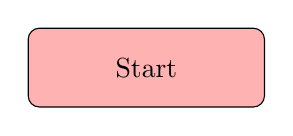
\begin{tikzpicture}[node distance=2cm]

\node (start) [startstop] {Start};

\end{tikzpicture}
%-----------------------------------------------------------------------------------------------------------------------
\subsection{Calculate}
\noindent
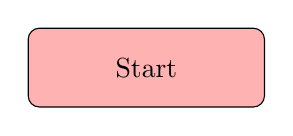
\begin{tikzpicture}[node distance=2cm]

\node (start) [startstop] {Start};

\end{tikzpicture}
%-----------------------------------------------------------------------------------------------------------------------
\subsection{Sort}
\noindent
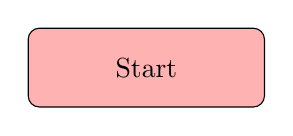
\begin{tikzpicture}[node distance=2cm]

\node (start) [startstop] {Start};

\end{tikzpicture}
%-----------------------------------------------------------------------------------------------------------------------
\subsection{Output}
\noindent
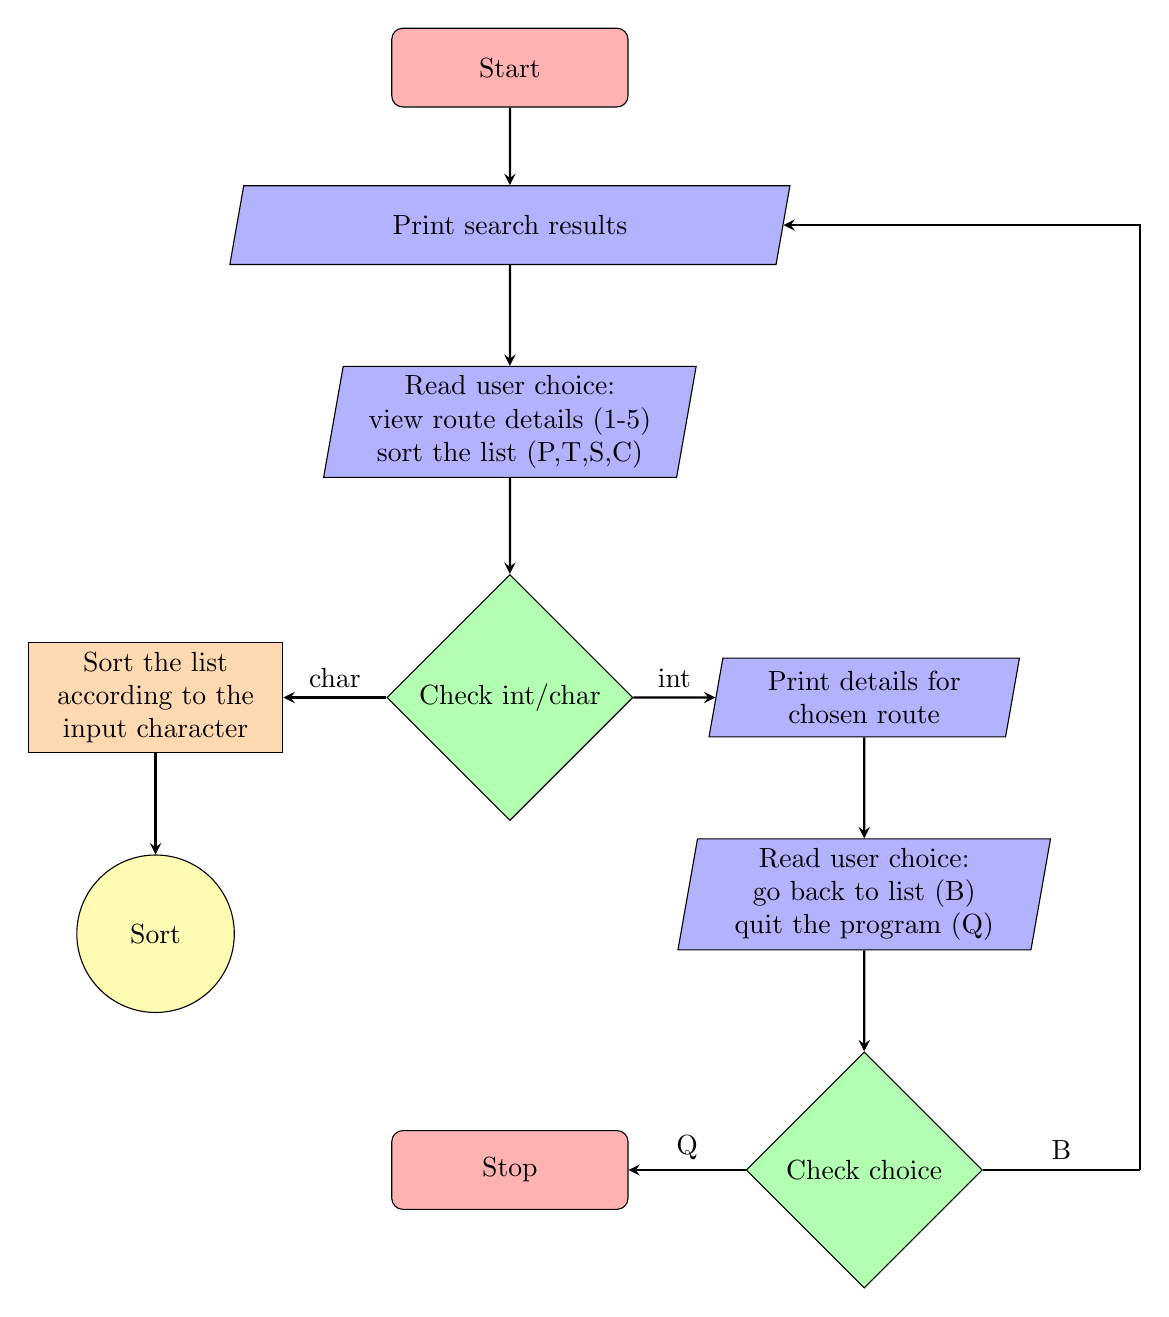
\begin{tikzpicture}[node distance=2cm]

\node (start) [startstop] {Start};
\node (out1)  [io, below of=start] {Print search results};
\node (in1)   [io, below of=out1, text width=4cm, yshift=-0.5cm] {Read user choice:\\ view route details (1-5)\\ sort the list (P,T,S,C)};
\node (dec1)  [decision, below of=in1, yshift=-1.5cm] {Check int/char};
\node (pro1)  [process, left of=dec1, xshift=-2.5cm] {Sort the list according to the input character};
\node (func1) [function, below of=pro1, yshift=-1cm] {Sort};
\node (out2)  [io, right of=dec1, xshift=2.5cm] {Print details for chosen route};
\node (in2)   [io, below of=out2, text width=4cm, yshift=-0.5cm] {Read user choice:\\ go back to list (B)\\ quit the program (Q)};
\node (dec2)  [decision, below of=in2, yshift=-1.5cm] {Check choice};
\node (stop)  [startstop, left of=dec2, xshift=-2.5cm] {Stop};

\coordinate [right of=dec2, xshift=1.5cm] (ph1);

\draw [arrow] (start) -- (out1);
\draw [arrow] (out1) -- (in1);
\draw [arrow] (in1) -- (dec1);
\draw [arrow] (dec1) -- node[anchor=south] {char} (pro1);
\draw [arrow] (pro1) -- (func1);
\draw [arrow] (dec1) -- node[anchor=south] {int} (out2);
\draw [arrow] (out2) -- (in2);
\draw [arrow] (in2) -- (dec2);
\draw [arrow] (dec2) -- node[anchor=south] {Q} (stop);
\draw [line] (dec2) -- node[anchor=south] {B} (ph1);
\draw [arrow] (ph1) |- (out1);

\end{tikzpicture}
%-----------------------------------------------------------------------------------------------------------------------
% textidote: ignore end

\section{Calculating the attributes}

Before we can properly print results in the program, we need to calculate the attributes of the different routes.
This is a relatively difficult task, as we need to calculate the distance, price, \unit{CO_{2}} and comfort.
Some attributes are easier to calculate than others, but they all require some form of calculation.

Rejseplanen has systems in place to calculate some of those attributes, but the API does not provide them.
This means that we have to calculate them ourselves.
Our calculations will not be 100\% accurate, but they will be close enough for our purposes.

\subsection{Calculating distance}

As we don't use a map API, we can't properly calculate the distance between two points.
This means that we have to ignore roads and instead calculate the distance by the train tracks.
The problem is that Rejseplanen only provides the coordinates of the stations, not the tracks.
So what we decided to do instead is to calculate the distance between the stations.
This won't account for curves along the track, as the distance is calculated as a straight line between the stations.
However, doing this for every station along the route is better than doing this for only the start and end station.
You can see an example of how the distance is going to look in Figure~\ref{fig:image-google-maps-distance-calculation}.

\begin{figure}[H]
    \centering
    \includegraphics[width=0.8\textwidth]{images/google-maps-distance-calculation.jpg}
    \caption{A route between Copenhagen and Odense. \\ Blue line is Google Maps' distance, black line is our distance.}
    % TODO fix the text not being centered
    \label{fig:image-google-maps-distance-calculation}
\end{figure}

% TODO Add explanation for how we calculate the distance

\subsection{Calculating price}

Calculating the price is a lot more difficult than calculating the distance.
As Denmark is divided into zones, the price is calculated based on how many zones you travel through.
The price is also affected based on a number of different variables, such as age, region, occupation and more.
For our program, we decided to calculate the prices for Pendlerkort and Ungdomskort.

\subsubsection{Zones}

First thing we need to do is to figure out how many zones a route goes through.
Unfortunately, Rejseplanen's API does not provide any information about how many zones a route goes through.
What we decided to do instead is to find the average size for a zone.
As the zones are not all the same size, the number of zones a route passes through may be slightly off.
But this is the best we can do with the current circumstances.

First we started by picking two stations and counted how many zones the route goes through using DSB's zone
map~\cite{price_zones}.
We then used Google Maps to calculate the distance along the tracks between two stations, and we noted it down.
Finally, we divided the distance by the number of zones to get the average size of a zone along the route.

\begin{figure}[H]
    \centering
    \noindent
    \begin{tabular}{ || c | c | c || }
        \hline
        Route & Zones and distance & Zone size \\
        \hline\hline
        Korsør to Ringsted & 5 zones 45 km & 9 km per zone \\
        \hline
        Ringsted to Køge Nord & 6 zones 30 km & 5 km per zone \\
        \hline
        Kalundborg to Holbæk & 7 zones 45 km & 6.4 km per zone \\
        \hline
        Frederikssund to Kbh & 10 zones 23 km & 2.3 km per zone \\
        \hline
        Voldingborg to Ringsted & 8 zones 52 km & 6.5 km per zone \\
        \hline\hline
        Zone Averages & & 6 km per zone \\
        \hline
    \end{tabular}
    \caption{Table of our calculations of zone size averages.}
    \label{fig:table-zone-size-averages}
\end{figure}

From Figure~\ref{fig:table-zone-size-averages} we determined that the average size of a zone is roughly about 6
kilometers.
But as you can see, the sizes of zones varies a lot.
This is unfortunate for us, as it means that the number of zones a route goes through may be inaccurate.

\subsubsection{Pendlerkort price}

The way we're going to calculate the price will is by figuring out the price for Pendlerkort.
This card allows commuters to freely travel between set amount of zones.
Rejseplanen has a website where the user can input their route, and it'll calculate the price for the
Pendlerkort~\cite{price_calculator}.
We then took the results and compared them to the price chart provided by DSB~\cite{price_sheet}.
Our calculations can be found in Figure~\ref{fig:table-rejseplanen-price-calculations} and
Figure~\ref{fig:image-dsb-pendlerkort-pris}.
The results are accurate enough that we deemed them good enough for our purposes.

\begin{figure}[H]
    \centering
    \noindent
    \begin{tabular}{ || c | c || }
        \hline
        Route & Zones and price \\
        \hline\hline
        Odense to København & 30 zones 3750 kr \\
        \hline
        Køge Nord to København & 9 zones 1470 kr \\
        \hline
        Græsted to Vordingborg & 18 zones 3000 kr \\
        \hline
        Aarhus to København & 51 zones 4590 kr \\
        \hline
    \end{tabular}
    \caption{Table of Rejseplanen's price calculations.}
    \label{fig:table-rejseplanen-price-calculations}
\end{figure}

\begin{figure}[H]
    \centering
    \includegraphics[width=1\textwidth]{images/dsb-pendlerkort-pris.jpg}
    \caption{Price of Pendlerkort per zones.}
    \label{fig:image-dsb-pendlerkort-pris}
\end{figure}

From what it seems, the price table is not recursive, so we can't implement a function to calculate the price.
Instead, we can save the table in the program and reference it when we need to find the price.
This allows us to have a pretty accurate price chart as long as the number of zones is accurate.

\subsubsection{Ungdomskort price}

Ungdomskort is a type op Pendlerkort that is primarily aimed at young people or students.
The price is significantly lower than Pendlerkort, so we deemed it necessary to implement it in our program.
The program would ask the user if they're a student, and if they are, the next calculation will be executed.
Calculating the price for Ungdomskort is a lot easier than Pendlerkort, as the method is listed on their
website~\cite{price_ung}.

The price is calculated by taking the equivalent price for a Pendlerkort and then taking 2487 kr from it.
Then the result is halved, and finally 663 kr is added to the result.
Here's an example for a Pendlerkort between Odense and Copenhagen, that costs 3750 kr:

\begin{equation}
    \frac{3750 - 2487}{2} + 663 = 1294 kr
\end{equation}

As a member in our group travels that same distance with an Ungdomskort, we can confirm that this result is accurate.

% textidote: ignore begin
\subsection{Calculating \unit{CO_{2}} emission}
% TODO Add the calculations, remove textiodte ignore
% textidote: ignore end

% textidote: ignore begin
\subsection{Calculating comfort value}
% TODO Add the calculation, remove textiodte ignore
% textidote: ignore end

\section{Saving user preferences}\label{sec:saving-user-preferences}

To make our program more user-friendly, we want to be able to store a users preferences on climate, price,
time, and so on.
This will be stored locally in a configuration file, which we will call
``\verb|preferences.json|''.
As the name suggests we have chosen to store the data in a JSON format, this is partly because we already have
a system in place in order to store JSON data, but also because it allows us to access individual keys of data such as
``price''.
If implemented correctly storing the preferences as JSON also allows us to remove or add different keys to the file
later if it is needed, but at this point we only need to save four keys called: price, time, environment and health.

For the actual implementation for saving the file.
We will, if the program is executed, always require data for all our chosen preference categories.
A way to do this is to, at the programs start, initialize the save file with some standard data, so the program can
continue running even if the user does not want to input their own preferences.
We initialize the save file through a function called ``InitializePreferenceFile''

\begin{figure}
    \centering
    \includegraphics[width=\textwidth]{InitPref}
    \caption{Saving preferences to file.}
    \label{fig:figureInitSaveFile}
\end{figure}

In Figure~\ref{fig:figureInitSaveFile} it can be seen that we are trying to open the preferences file,
and by using ``fopen'' we make use of the property that creates the file if it does not already exist.
The rest of the code inside InitializePreferenceFile is used to convert our given inputs into the JSON format, which in
C is somewhat difficult.

The remaining functions for the preference file are SetUserPreference and GetUserPreference.
The SetUserPreference function will work by taking in two inputs, a key and a value for that key.
This would be written as \(SetUserPreference("key", value)\).
When we want to change the values in the JSON file through C, we must first read the file and then parse it as cJSON[.]
In this way we can actually make the changes to the stored values.
Parsing JSON and generating JSON is done through the library cJSON which we have chosen to use.
As seen above it works by first parsing the content of the preference file and then searching for the item we want to
change.

\begin{figure}
    \centering
    \includegraphics[width=\textwidth]{ParsingJSON}
    \caption{Parsing JSON.}
    \label{fig:figureParsingJSON}
\end{figure}

cJSON stores all JSON values as structs and to change the value we access the struct as seen on line 82 in
Figure~\ref{fig:figureParsingJSON}.
The next step is then to save the changes to our preferences file, but because saving to a file in C can get
complicated if you change the length of the file, we sidestep this problem by overwriting the whole save file with the
updated values.

Finally, the last step is to read the file, so we can use the stored data in our program.
This is done much in the same way we used in SetUserPreference as we open the file, parse the JSON and then access
the item we want to use.
Both InitializePreferenceFile and SetUserPreference are void functions, but GetUserPreference is a double function
this is done so the returned value will be the value for the preference we want to get out of the save file, see
Figure~\ref{fig:figureGetPref}.
GetUserPreference only takes in one input which is the key we want to look for, this could be ``price'' or another of
the attributes.

\begin{figure}
    \centering
    \includegraphics[width=\textwidth]{GetPref}
    \caption{Reading attribute value from preference file.}
    \label{fig:figureGetPref}
\end{figure}

With these three functions it is now possible for us to store and use preferences locally on the device.



    \bibliographystyle{IEEEtran}
    % textidote: ignore begin
    \bibliography{problem-analysis/audience,problem-analysis/existing-solutions,problem-analysis/financial-awareness,
        problem-analysis/health,problem-analysis/history,problem-analysis/what-is-the-problem,
        method/software-project-structure,method/solution-stack}
    % textidote: ignore end
\end{document}
